
\section{Introduction to the Architecture}

\subsection{Abstract Hardware Architecture}

For proper understanding of openETCS \gls{API} and of constraints imposed on
both sides of the \gls{API}, we need to define a \define{reference abstract hardware architecture}. This hardware architecture is ``abstract''
is the sense that the actual vendor specific hardware architecture
might be totally different of the abstract architecture described in
this chapter. For example, several units might be grouped together on
the same processor.

However the actual vendor specific architecture shall fulfil all the
requirements and constraints of this reference abstract hardware
architecture and shall not request additional constraints.

\subsection{Definition of the reference abstract hardware architecture}

\begin{figure}
  \centering
  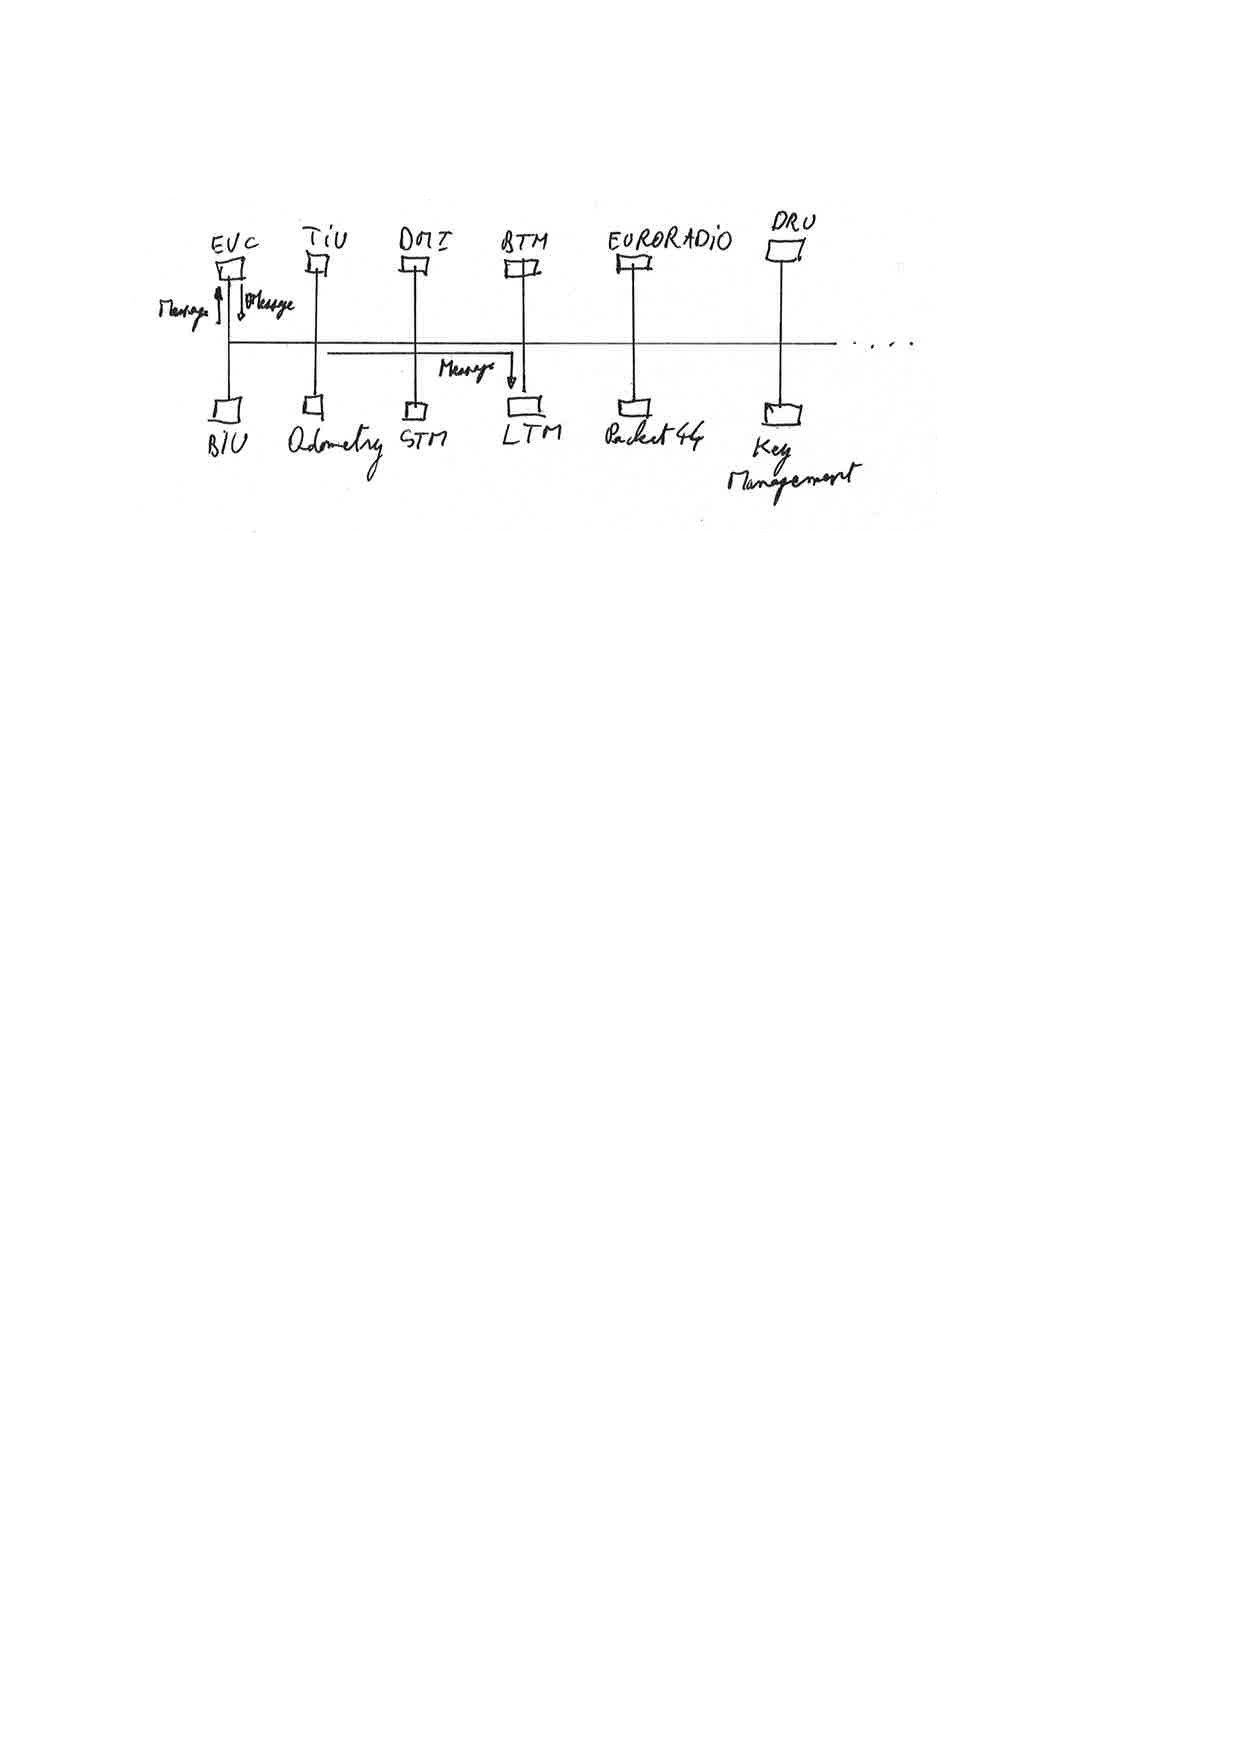
\includegraphics[width=\linewidth]{abstract-hardware-architecture.pdf}
  \caption{Reference abstract hardware architecture}
  \label{fig:hardware-arch}
\end{figure}

The reference abstract hardware architecture is shown in figure
\ref{fig:hardware-arch}.

The reference abstract hardware architecture is made of a bus on which
are connected \define{units} defining the \gls{OBU}:

\begin{itemize}
\item \gls{EVC};
\item \gls{TIU};
\item \gls{ODO};
\item \gls{DMI};
\item \gls{STM};
\item \gls{BTM};
\item \gls{LTM}: Not part of this openETCS implementation;
\item EURORADIO;
\item \gls{JRU}: Not part of this openETCS implementation;
\end{itemize}

Elements not being part of this implementation are marked. 

Those units shall working concurrently. They shall exchange
information with other units through asynchronous message passing.

\subsection{Reference abstract software architecture}
\label{software-arch}

\begin{figure}[htbp]
  \centering
  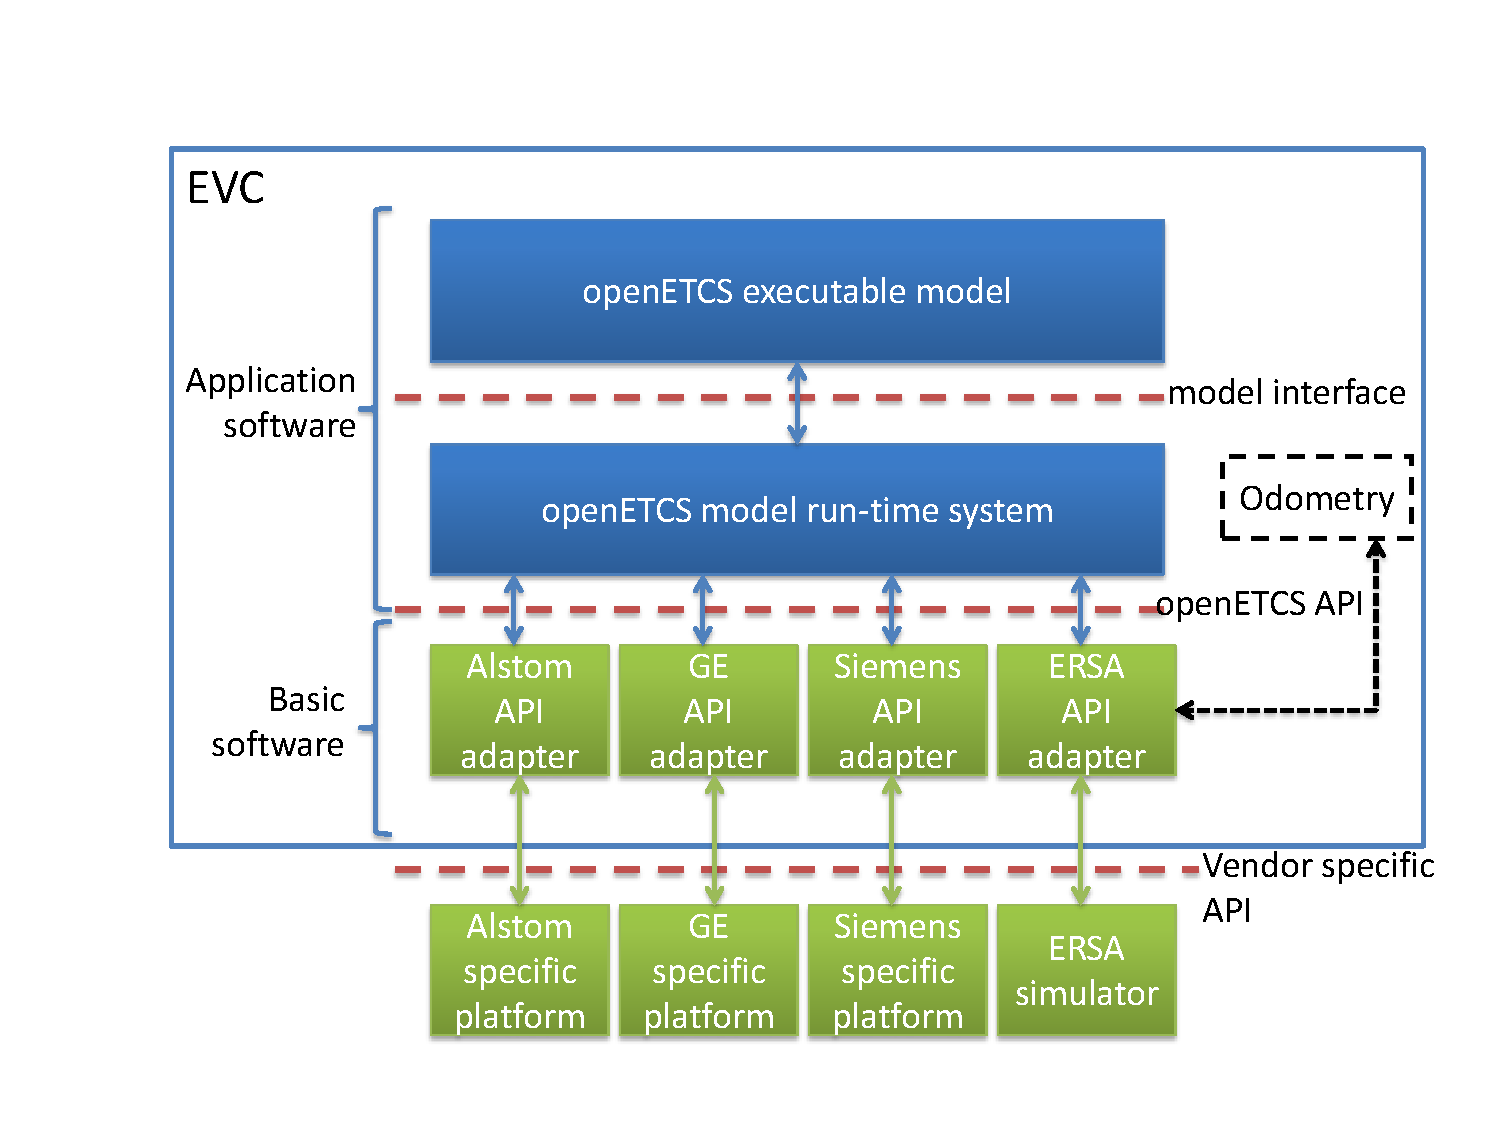
\includegraphics[width=\linewidth]{software-architecture.pdf}
  \caption{Reference abstract software architecture}
  \label{fig:software-arch}
\end{figure}

The \define{reference abstract software architecture} is shown in figure
\ref{fig:software-arch}. This architecture is made of following
elements:
\begin{itemize}
\item \define{openETCS executable model} produced by the
  \cite{scade-model} Scade Model. It shall contain the program implementing core
  ETCS functions;
\item\define{openETCS model run-time system} shall help the execution
  of the openETCS executable model by providing additional functions
  like encode/decode messages, proper execution of the model through
  appropriate scheduling, re-order or prioritize messages, etc. 
\item \define{Vendor specific \gls{API} adapter} shall make the link between
  the Vendor specific platform and the openETCS model run-time system.
  It can buffer message parts, encode/decode messages, route messages
  to other \gls{EVC} components, etc.
\item All above three elements shall be included in the \gls{EVC};
\item \define{Vendor specific platform} shall be all other elements of
  the system, bus and other units, as shown in figure
  \ref{fig:hardware-arch}.
\end{itemize}

We have thus three interfaces:
\begin{itemize}
\item \define{model interface}
 is the interface between openETCS
  executable model and openETCS model run-time system. 
\item \define{openETCS \gls{API}}
 is the interface between openETCS model
  run-time system and Vendor specific \gls{API} adapter.
\item \define{Vendor specific \gls{API}}
 is the interface between Vendor
  specific \gls{API} adapter and Vendor specific platform. This interface is
  not publicly described for all vendors. You can find the Alstom imnplementation as an example.
\end{itemize}

The two blocks openETCS executable model and openETCS model run-time
system are making the \define{Application software} part. This Application software might be either openETCS reference software or
vendor specific software.

The Vendor specific \gls{API} adapter is making the \define{Basic software} part.


\section{Functional breakdown}


\subsection{F1: openETCS \gls{API} Runtime System and Input to the EVC)}
\label{chp_openETCS_API}
%Authors: Bernd Hekele (DB)

\begin{figure}[hbtp]
\centering
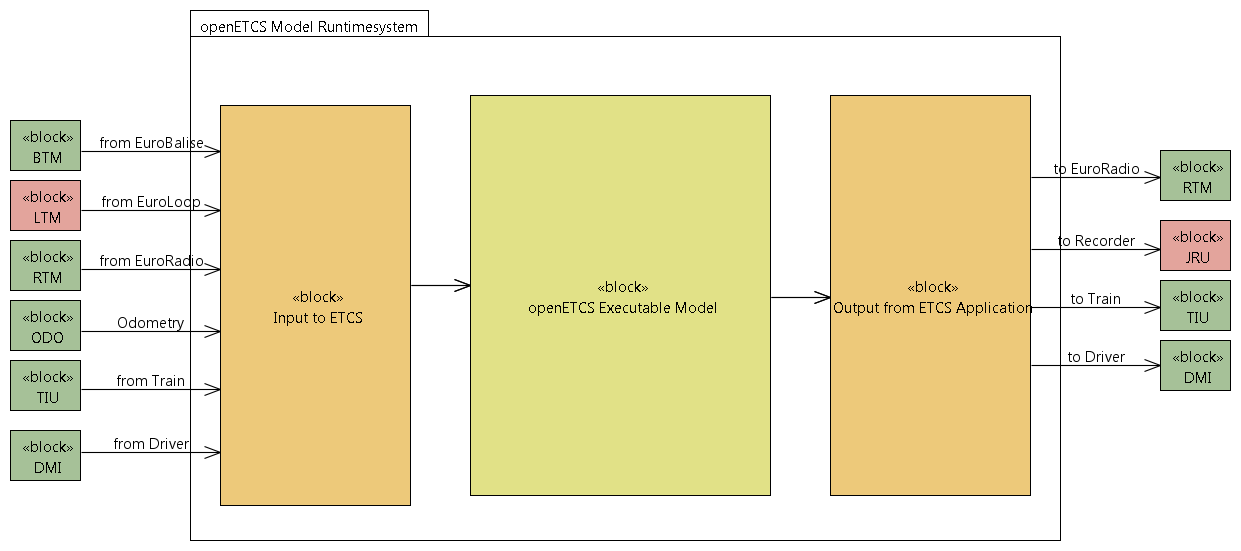
\includegraphics[width=\linewidth]{openETCSAPI.png}
\caption{openETCS API Highlevel View}
\label{fig:apiHighLevel}
\end{figure}

Figure \ref{fig:apiHighLevel} shows the structure of API with respect of the software architecture. Input boxes and output boxes not implemented in this stage are marked as red, other interfaces are marked as green. The System covers functions for processing Inputs from other Units, functions for processing Outputs to other functions and a basic runtime system. Inputs are used to feed the input to the executable model before calling it, outputs are used for collecting information provided by the executable model to be passed to the relevant interfaces after the execution cycle has finished.

\subsubsection{Principles for Interfaces (openETCS \gls{API})}


Information  is exchanged \define{messages} in an asynchronous way. A message is a set
of information corresponding to an event of a particular unit, e.g. a
balise received from the \gls{BTM}. The possible kind of messages are
described in chapter \ref{information-flows}.

The information is passed to the executable model as parmeters to the snychronous call of a procedure (Interface to the executable model). Since the availability of input messages to the application is not guaranteed the parts of the interfaces are defined with a "present" flag. In addition, fields of input arraysquite often is of variable size. Implementation in the concrete interface in this use-case is the use of a "size" parameter and a "valid"-flag.


\subsubsection{openETCS Model Runtime System}
The openETCS model runtime system also provides:

\begin{itemize}
\item Input Functions From other Units\\
In this entity messages from other connected units are received.
\item Output Functions to other Units\\
The entity writes messages to other connected units.
\item Conversation Functions for Messages (Bitwalker)\\
The conversion function are triggered by Input and Ouput Functions. The main task is to convert input messages from an bit-packed format into logical ETCS messages (the ETCS language) and Output messages from Logical into a bit-packed format. The logical format of the messages is defined for all used types in the openETCS data dictonary. \\
Variable size elements in the Messages are converted to fixed length arrays with an used elements indicator.\\
Optional elements are indicated with an valid flag.
The conversion routines are responsible for checking the data received is valid. If  faults are detected the information is passed to the openETCS executable model for further reaction. 
\item Model Cycle\\

The version management function is part of the message handling.This implies, conversions from other physical or logical layouts of messages are mapped onto a generic format used in the EVC. Information about the origin version of the message is part of the messages.
 
The executable model is called in cycles. In the cycle 
\begin{itemize}
\item First the received input messages are decoded
\item The input data is passed to the executable model in a predefined order. \textbf{(Details for the interface to be defined)}.
\item Output is encoded according to the \gls{SRS} and passed to the  buffers to the units.
\end{itemize}
\end{itemize}


\subsubsection{Input Interfaces of the openETCS API From other Units of the OBU}
Interfaces are defined in the Scade project APITypes (package API\_Msg\_Pkg.xscade).

In the interfaces the following principles for indicating the quality of the information is used:


\tablefirsthead{
\hline 
\rowcolor{gray} 
Indicator & Type & Purpose \\\hline}
\begin{supertabular}{| p{2 cm} | p{2 cm} | p{8 cm} |}
present & bool & True indicates the component has been changed compared to the previous call of the routine
\\\hline 
valid & bool & True indicates the component is valid to be used. 
\\\hline 
\end{supertabular}

In the next table we can see the interfaces being used in the openETCS system. Details on the interfaces are defined further down.

\tablefirsthead{
\hline 
\rowcolor{gray} 
Unit & Name &  Processing Function  \\\hline}
%\begin{itemize}{| m{1.2cm} | m{1.5cm} | m{1.2cm} | m{3.7cm}  | m{3.7cm} |}
\begin{supertabular}{| c | c | c |}
\gls{BTM} & Balise Telegram & Receive Messages  \\\hline
\gls{DMI} & Driver Machine Interface & DMI Manager  \\\hline
EURORADIO & Communication Management & Communication Management  \\\hline
EURORADIO & Radio Messages & Receive Messages  \\\hline
\gls{ODO} & Odometer & All Parts \\\hline
System TIME & Time system of the OBU & All Parts \\\hline
TIU & Train Data & All Parts \\\hline
\end{supertabular}

Information in the following sections gives an more detailed overview of the structure of the interfaces.


\subsubsection{Message based interface (BTM, RTM)}


Balise Message (Track to Train)\\

\tablefirsthead{
\hline 
\rowcolor{gray} 
Message Name & Optional Packets & Restrictions in the current scope \\\hline}
\begin{supertabular}{| p{4 cm} | p{6 cm} | p{4,5 cm} |}
Balise Telegram &
3: National Values \newline
41: Level Transition Order \newline
42: Session Management  \newline
45: Radio Network registration \newline
46: Conditional Level Transition Order \newline
65: Temporary Speed Restriction \newline
66: Revoke Temporary Speed Restriction \newline
72: Packet for sending plain text messages \newline
137: Stop if in Staff Responsible \newline
255: End of Information \newline
& Used in Scenario
\\\hline
Balise Telegram &
0, 2, 3, 5, 6, 12, 16, 21, 27, 39,
40, 41, 42, 44, 45, 46, 49, 51, 52, 65,
66, 67, 68, 69, 70, 71, 72, 76, 79, 80,
88, 90, 131, 132, 133, 134, 135, 136, 137, 138,
139, 141, 145, 180, 181, 254
&  Not Used in Scenario\\\hline
\end{supertabular}

Radio Messages (Track to Train)

\tablefirsthead{
\hline 
\rowcolor{gray} 
Message Name & Optional Packets & Restrictions in the current scope \\\hline}
\begin{supertabular}{| p{4 cm} | p{6 cm} | p{4,5 cm} |}
2: SR Authorisation & 63:\ List\ of\ Balises\ in\ SR Authority & Message Not Supported \\\hline
3: Movement Authority &
 21:\ Gradient\ Profile\newline
 27: International Static Speed Profile\newline
 49: List of balises for SH Area\newline
 80: Mode profile\newline
 plus common optional packets\newline
 & a \\\hline
9: Request To Shorten MA &
 49: List of balises for SH Area\newline
 80: Mode profile\newline 
& \\\hline
24: General Message &
From RBC:\newline
 21:\ Gradient\ Profile\newline
 27: International Static Speed Profile\newline
 plus common optional packets\newline
From RIU:\newline 44, 45, 143, 180, 254
& Messages from RIU are not supported \\\hline
28: SH authorised & 3, 44, 49
& \\\hline
33: MA with Shifted Location Reference &
 21:\ Gradient\ Profile\newline
 27: International Static Speed Profile\newline
 49: List of balises for SH Area\newline
 80: Mode profile\newline
 plus common optional packets\newline
& \\\hline
37: Infill MA &
5, 21, 27, 39, 40, 41, 44, 49, 51, 52, 65, 66, 68, 69, 70, 71, 80, 88, 138, 139 
 & Message Not Supported \\\hline
List of common optional parameters &
3, 5, 39, 40, 51, 41, 42, 44, 45, 52, 57, 58, 64, 65, 66, 68, 69, 70, 71, 72, 76, 79, 88, 131, 138, 139, 140, 180
& \\\hline
\end{supertabular}

The runtime system is in charge to transfer the messages from its stream mode first to  compressed message format. 

\subsubsection{Interfaces to the Time System}
The interface types are defined in the OBU\_Basic\_Types\_Pkg Package. The system time is defined in the basic software.

The system TIME is provided to the executable model at the begin of the cycle. It is not refreshed during the cycle. The time provided to the application is equal to 0 at power-up of the EVC (it is not a “UTC time” nor a “Local
Time”), then must increase at each cycle (unit = 1 msec), until it reaches its maximum value (i.e current EVC
limitation = 24 hours)

\begin{itemize}
\item TIME (T\_internal\_Type, 32-bit INT)\\
Standardized system time type used for all internal time calculations: in ms. The time is defined as a cyclic counter: When the maximum is exceeded the time starts from 0 again. 

\item CLOCK (to be implemented)\\
The clocking system is provided by the JRU. A GPS based clock is assumed to provide the local time.

\end{itemize}

\subsubsection{Interfaces to the Odometry System}
The interface types are defined in the OBU\_Basic\_Types\_Pkg Package. 
The odometer gives the current information of the positing system of the train. In this section the structure of the interfaces are only highlighted. Details, including the internal definitions for distances, locations speed and time are implemented in the package. 

\begin{itemize}
\item Odometer (odometry\_T)
\begin{itemize}
\item valid (bool)\\
valid flag, i.e., the information is provided by the ODO system and can be used.
\item timestamp (T\_internal\_Type)\\
of the system when the odometer information was collected. Please, see also general remarks on the time system. 
\item Coordinate (odometryLocation\_T)
\begin{itemize}
\item nominal (L\_internal\_Type) [cm]
\item min (L\_internal\_Type) [cm]
\item max (L\_internal\_Type) [cm]
\end{itemize}
The type used for length values is a 32 bit integer. 
Min and max value give the interval where the train is to be expected. The bounderies are determined by the inaccuracy of the positioning system. All values are set to 0 when the train starts.

\item speed (OdometrySpeeds\_T) [km/h]
\begin{itemize}
\item v\_safeNominal (speed internal type) [km/h]\\
The safe nominal estimation of the speed which will
be bounded between 98\% and 100\% of the upper
estimation
\item v\_rawNominal (speed internal type) [km/h]\\
The raw nominal estimation of the speed which will
be bounded between the lower and the upper
estimations
\item v\_lower (speed internal type) [km/h]\\
The lower estimation of the speed
\item v\_upper (speed internal type) [km/h]\\
The upper estimation of the speed
\end{itemize}
The type used for speed values is a 32 bit integer. 
Min and max value give the interval where the train is to be expected. The bounderies are determined by the inaccuracy of the positioning system. All values are set to 0 when the train starts.
\item acceleration (A\_internal\_Type)[0.01 m/s2],\\
Standardized acceleration type for all internal calculations : in 
\item motionState (Enumeration)\\
indicates whether the train is in motion or in no motion
\item motionDirection (Enumeration)\\
indicates the direction of the train, i.e., CAB-A first, CAB-B first or unknown.
\end{itemize}
\end{itemize}

\subsubsection{Interfaces to the Train Interfaces (TIU)}
The following infomration is based on the implementation of the Alstom API. The interface is organised in packets. The packets of the Alstom implementation are listed in the appendix to this document.

The description of interfaces needed for the current scope will be added according to the use.

\subsubsection{Output Interfaces of the openETCS API TO other Units of the OBU}

\tablefirsthead{
\hline 
\rowcolor{gray} 
From Function & Name &  To Unit & Description \\\hline}
%\begin{supertabular}{| m{1.2cm} | m{1.5cm} | m{1.2cm} | m{3.7cm}  | m{3.7cm} |}
\begin{supertabular}{| c | c | c | c  | c |}
 & Radio Output Message & \ EURORADIO & \\\hline
 & Communication Management  &  EURORADIO  & \\\hline
 & Driver Information & \gls{DMI} & \\\hline
 & Train Data  & TIU &  
\\\hline
\end{supertabular}

Packets:
to be completed

Radio Messages
to be completed


%-----------------------------------------------------------------------
%\subsection{Runtime- APIl}
%-----------------------------------------------------------------------
%\tbc
%JakobGärtner
